\documentclass[10pt, a5paper]{article}
\usepackage{pdfpages}
\usepackage{parallel}
\usepackage[T2A]{fontenc}
\usepackage{ucs}
\usepackage[utf8x]{inputenc}
\usepackage[polish,english,russian]{babel}
\usepackage{hyperref}
\usepackage{rotating}
\usepackage[inner=2cm,top=1.8cm,outer=2cm,bottom=2.3cm,nohead]{geometry}
\usepackage{listings}
\usepackage{graphicx}
\usepackage{wrapfig}
\usepackage{longtable}
\usepackage{indentfirst}
\usepackage{array}
\newcolumntype{P}[1]{>{\raggedright\arraybackslash}p{#1}}
\frenchspacing
\usepackage{fixltx2e} %text sub- and superscripts
\usepackage{icomma} % коскі ў матэматычным рэжыме
\PreloadUnicodePage{4}

\newcommand{\longpage}{\enlargethispage{\baselineskip}}
\newcommand{\shortpage}{\enlargethispage{-\baselineskip}}

\def\switchlang#1{\expandafter\csname switchlang#1\endcsname}
\def\switchlangbe{
\let\saverefname=\refname%
\def\refname{Літаратура}%
\def\figurename{Іл.}%
}
\def\switchlangen{
\let\saverefname=\refname%
\def\refname{References}%
\def\figurename{Fig.}%
}
\def\switchlangru{
\let\saverefname=\refname%
\let\savefigurename=\figurename%
\def\refname{Литература}%
\def\figurename{Рис.}%
}

\hyphenation{admi-ni-stra-tive}
\hyphenation{ex-pe-ri-ence}
\hyphenation{fle-xi-bi-li-ty}
\hyphenation{Py-thon}
\hyphenation{ma-the-ma-ti-cal}
\hyphenation{re-ported}
\hyphenation{imp-le-menta-tions}
\hyphenation{pro-vides}
\hyphenation{en-gi-neering}
\hyphenation{com-pa-ti-bi-li-ty}
\hyphenation{im-pos-sible}
\hyphenation{desk-top}
\hyphenation{elec-tro-nic}
\hyphenation{com-pa-ny}
\hyphenation{de-ve-lop-ment}
\hyphenation{de-ve-loping}
\hyphenation{de-ve-lop}
\hyphenation{da-ta-ba-se}
\hyphenation{plat-forms}
\hyphenation{or-ga-ni-za-tion}
\hyphenation{pro-gramming}
\hyphenation{in-stru-ments}
\hyphenation{Li-nux}
\hyphenation{sour-ce}
\hyphenation{en-vi-ron-ment}
\hyphenation{Te-le-pathy}
\hyphenation{Li-nux-ov-ka}
\hyphenation{Open-BSD}
\hyphenation{Free-BSD}
\hyphenation{men-ti-on-ed}
\hyphenation{app-li-ca-tion}

\def\progref!#1!{\texttt{#1}}
\renewcommand{\arraystretch}{2} %Іначай формулы ў матрыцы зліпаюцца з лініямі
\usepackage{array}

\def\interview #1 (#2), #3, #4, #5\par{

\section[#1, #3, #4]{#1 -- #3, #4}
\def\qname{LVEE}
\def\aname{#1}
\def\q ##1\par{{\noindent \bf \qname: ##1 }\par}
\def\a{{\noindent \bf \aname: } \def\qname{L}\def\aname{#2}}
}

\def\interview* #1 (#2), #3, #4, #5\par{

\section*{#1\\{\small\rm #3, #4. #5}}

\def\qname{LVEE}
\def\aname{#1}
\def\q ##1\par{{\noindent \bf \qname: ##1 }\par}
\def\a{{\noindent \bf \aname: } \def\qname{L}\def\aname{#2}}
}

\switchlang{en}
\begin{document}
\title{Yocto and OpenEmbedded at Collabora}
\author{Andrew Shadura, Bratislava, Slovakia}
\maketitle
\begin{abstract}
How the use of Yocto and OpenEmbedded helps corporations migrate to free software
\end{abstract}

There's a certain confusion existing even among people closely \linebreak working with Yocto Project, on what exactly Yocto is. First of all, Yocto isn't a Linux distribution. In fact, Yocto Project is an umbrella organisation that takes care of a bunch of embedded Linux technologies, including OpenEmbedded Core, BitBake, Poky and others. These and others technologies Yocto Project provides allow users to build custom Linux distributions suited to their own needs.

One might ask, if Yocto isn't a distribution, how does one make a distribution using its technologies?

\begin{figure}[h!]
  \centering
  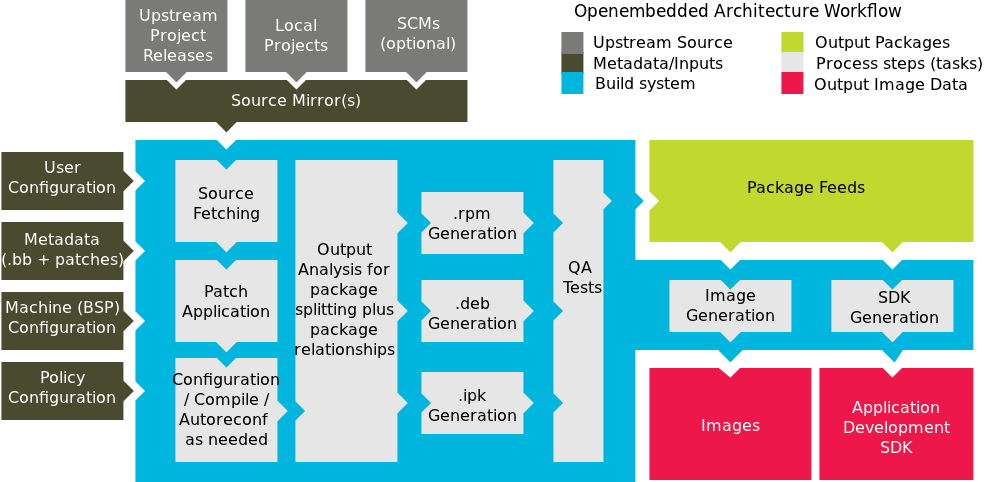
\includegraphics[height=5.5cm]{w_07_2016_Shadura1.png}
\end{figure}

The current Yocto technology stack has evolved from its roots in previously separate OpenEmbedded Project. Since the merger \linebreak of OpenEmbedded and Yocto, OpenEmbedded has introduced a layers system allowing vendors and users to have their bits separate yet \linebreak plugging into each other. There's a number of layers Yocto Project provides ({\ttfamily oe-core, meta-yocto, meta-yocto-bsp}) which form so-called \linebreak <<reference distribution>>, Poky. Poky contains foundation package \linebreak recipes (from OpenEmbedded Core), distribution policy\linebreak configuration, reference BSPs, build tools and documentation. Normally, Poky is what you start from when creating your own distribution.

\begin{figure}[h!]
  \centering
  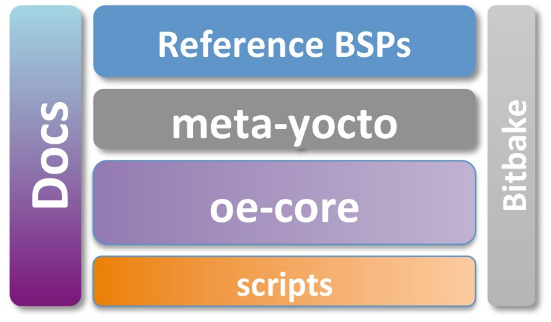
\includegraphics[height=5.5cm]{w_07_2016_Shadura2.png}
\end{figure}

Package recipes are written in a language similar to both Make and shell, and to certain extent resemble Gentoo's ebuilds. These recipes are being used by BitBake to build binary packages, and provide necessary information on where sources are found, and how to build them. BitBake recipes support includes, inheritance and overrides making it easy to change or extend the behaviour of an existing recipe without touching its code.

\begin{figure}[H]
  \centering
  
\includegraphics[width=10cm]{w_07_2016_Shadura3.png}
  \caption* {Fig: Example of a BitBake recipe.}
\end{figure}

\begin{figure}[H]
  \centering
  
\includegraphics[width=10cm]{w_07_2016_Shadura4.png}
  \caption* {Fig: Example of a BitBake recipe with inheritance}
\end{figure}

\begin{figure}[H]
  \centering
  
\includegraphics[height=2.5cm]{w_07_2016_Shadura5.png}
  \caption* {Fig: Example of .bbappend}
\end{figure}


Collabora is a company that provides consultancy to companies who are deploying open source technologies in their products, by providing its own open source based products and through knowledge sharing activities such as training. Collabora employs many free software \linebreak developers who are experts or major developers in such areas as \linebreak multimedia (GStreamer), graphics (Wayland, Weston), Linux kernel, productivity software (LibreOffice) and others.

At Collabora, we use Yocto on a project for a manufacturer of medical equipment, who use a Linux-based operating system in their products. Currently, their production devices are using a very custom Buildroot-based system, which runs quite an old (3.x-something) version of Linux kernel with lots of custom proprietary daemons and APIs. At some point they realised that it's quite a difficult task to support that system, and they decided they need help of experts, us.

For the project, the customer have decided to eliminate as much as possible custom proprietary libraries, take as much work as possible upstream, migrate to and integrate systemd as the init system. They also wanted us to help them with development methodology.

Thanks to the layer system Yocto Project uses, building your own distribution based on it is quite an easy job, once you know what you need from it. It all started as a layer with three files: the layer definition itself, distribution configuration file, and a machine definition.

\begin{figure}[h!]
  \centering
  
\includegraphics[height=5.5cm]{w_07_2016_Shadura6.png}
  \caption* {Fig: Layer definition file (conf/layer.conf)}

\end{figure}

\begin{figure}[h!]
  \centering
  
\includegraphics[width=10cm]{w_07_2016_Shadura7.png}
  \caption* {Fig: Distribution definition file (conf/distro/badger.conf)}
\end{figure}

\begin{figure}[h!]
  \centering
  
\includegraphics[width=10cm]{w_07_2016_Shadura8.png}
  \caption* {Fig: Machine definition file (conf/machine/vexpressa9.conf)}
\end{figure}


These files define where recipe files are to be found, exactly what features (systemd, wayland, apparmor) we're using and what we don't (x11, sysvinit), and what processor architectures we're building for, what types of images we need to generate and so on.

For architecture-dependent parts, we first used a layer Freescale provided (meta-fsl-arm, meta-fsl-arm-extra), so we wouldn't need to write our own image generation routines, or tuning the cross-compiler features by hand. Later, we removed that dependency by bundling greatly simplified and customised versions of Freescale's recipes, but until we needed that it was a great help that we could reuse already working code.

When the initial phase of the project was completed, and we had a working image booting on a hardware prototype with Weston shell running, it was decided to split our layer in two, thus separating the platform itself and the application layer. Into the application layer went customer's proprietary software that will remain proprietary — at least, for now, and supporting daemons and libraries it depends on. The platform layer is almost entirely free software, with the exception of a few legacy hardware-related daemons which will be at some point replaced with their free software counterparts.

One might ask, why do we need anything in the platform layer apart from the distro configuration, if it's free software anyway? The answer is that, we're using quite some bleeding edge technology packages, but at the same time we want our platform to be based on the stable branch of Poky, the Yocto meta-distribution. That means, from time to time we need to import recipes for newer versions of software from the development branch. This is especially true when recipes coming from Yocto need to be improved: while BitBake allows extending existing recipes with use of .bbappend files, we mostly use that for distribution-specific things only. If we need some generic change that can be upstreamed, like user sessions support in systemd and dbus, we copy the latest version of the recipe from upstream, and patch it locally, so that the fixes can be easily submitted upstream.

This brings a benefit of needing minimal edits to the patches before they're submitted; otherwise we'd need a complete rewrite of the feature we need.

Apart from software updates and patches we also carry recipes for some free software which isn't release-ready, some custom configuration and some temporary workarounds for kernel bugs we don't currently have capacity to fix properly.

So far, since the project began, our team has contributed to the community at least the following:

\begin{itemize}
  \item lots of fixes to various OE Core package recipes, including patches enabling systemd integration, merged /usr
  \item patches to Weston and Linux kernel enabling accelerated graphics on our hardware
  \item patches to ifupdown adding inheritance feature similar to what BitBake has
  \item lot more
\end{itemize}

Kernel support for the customer's hardware is all being upstreamed by the customer, as the customer believes their hardware should run mainline kernel.

Even though the project is still in progress, even at its current stage it clearly demonstrates how is possible to migrate a big project to an open platform, reducing the maintenance cost and at the same time helping everyone else, and to a great extent that is possible thanks to Yocto.

\end{document}
